
\section{The resulting game}
The end result is a playable arkanoid game. Upon starting the game, the ASCII art title screen
shown in figure \ref{title} is displayed. After proceeding from the title screen, the first
level starts and the player can control the striker using a potmeter connecting to the eZ8
development board. In figure \ref{screenshots} a few screenshots from the game can be seen. \\

The game is very hard and unforgiving as you start with a score of zero and lose 25 points every
time you miss the ball. However the skill need to complete the game can quickly be
aquired. \\

The game runs at 30 frames per second without skipping frames, which makes for a very
smooth visual experience. The song "Popcorn" plays in the background, and every time
the ball hits a brick, a border or the striker, a sound is played.
 The dark backgrounds function well with the high contrast
color of the ball and striker. If the player dies, he/she is presented with a screen
encouraging them to retry the game, if the user accepts the game will automatically restart.
If the player manages to win the game, he/she is presented with a win message and the final
score, as well as the option to play again.  It is hard to describe the gameplay apart from the
provided screenshots. The reader is encouraged to refer to the gameplay manual and
try playing the game. It should be noted that the game can only be played in the PuTTY terminal
due to the resolution and color use.

\begin{figure}
	\center
	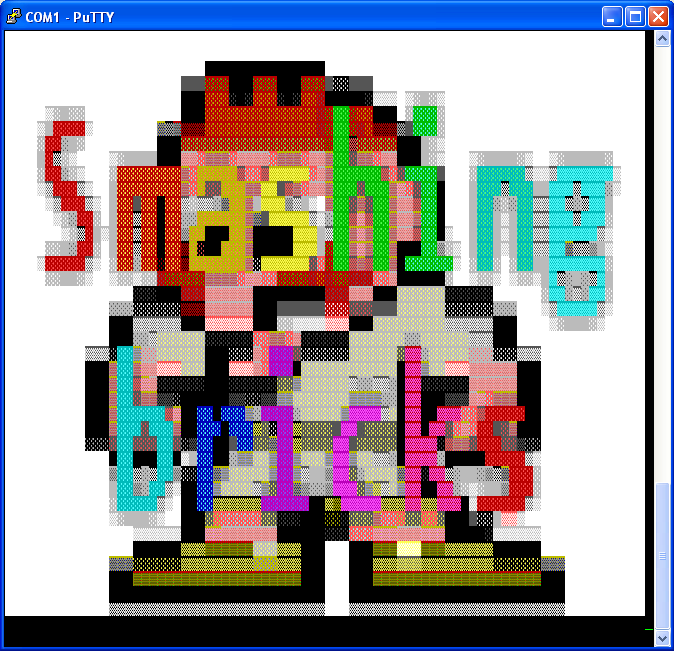
\includegraphics[scale=0.5]{pictures/title_screen.PNG}
	\caption{The Smashing Bricks title screen}
	\label{title}
\end{figure}

\begin{figure}
	\center
	\begin{subfigure}[t]{\columnwidth}
		\center
		\begin{subfigure}{0.3\linewidth}
			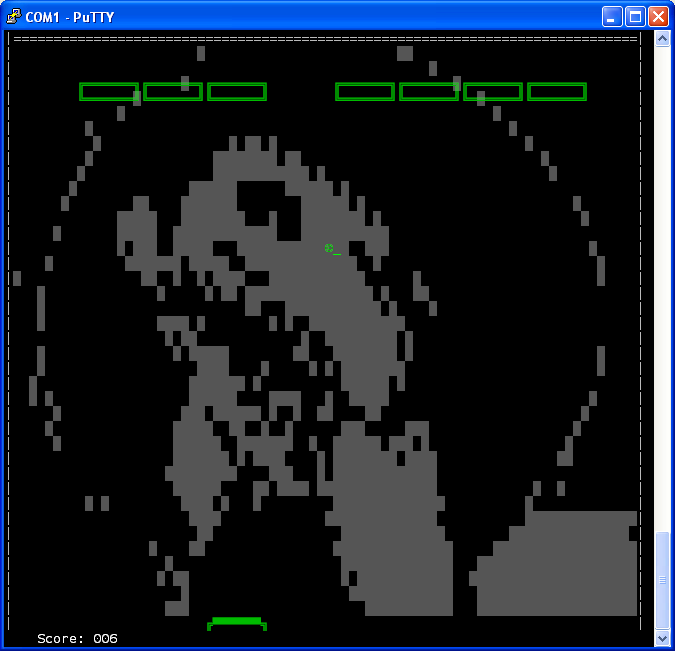
\includegraphics[scale=0.3]{pictures/level_1.PNG}
		\end{subfigure}
		\begin{subfigure}{0.3\linewidth}
			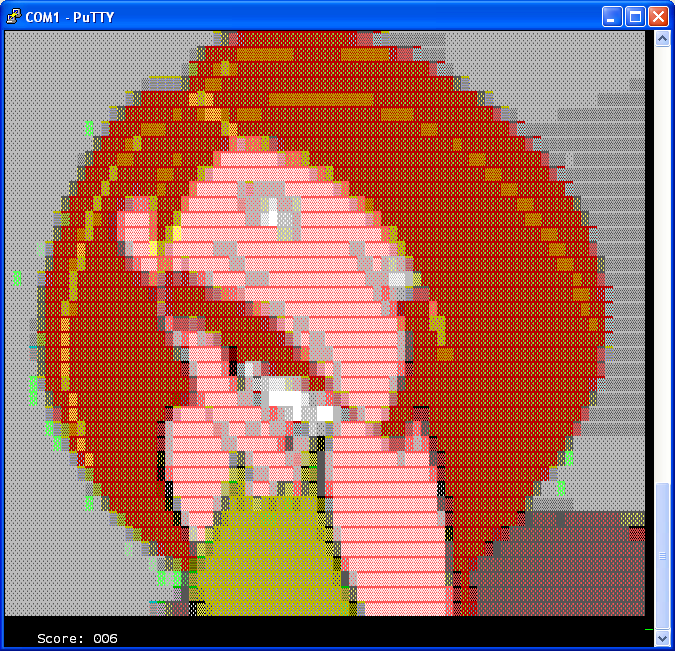
\includegraphics[scale=0.3]{pictures/level_1_complete.PNG}
		\end{subfigure}
		\begin{subfigure}{0.3\linewidth}
			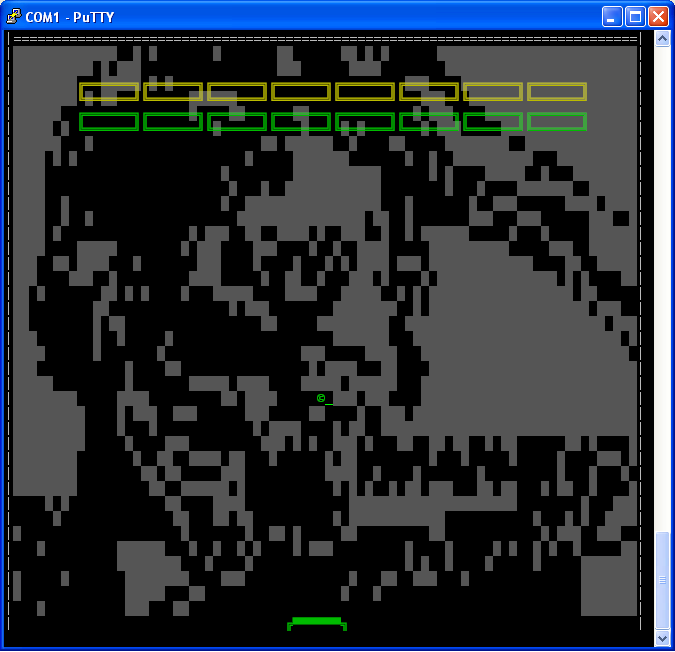
\includegraphics[scale=0.3]{pictures/level_2.PNG}
		\end{subfigure}
	\end{subfigure}
	\begin{subfigure}[c]{\columnwidth}
		\center
		\begin{subfigure}{0.3\linewidth}
			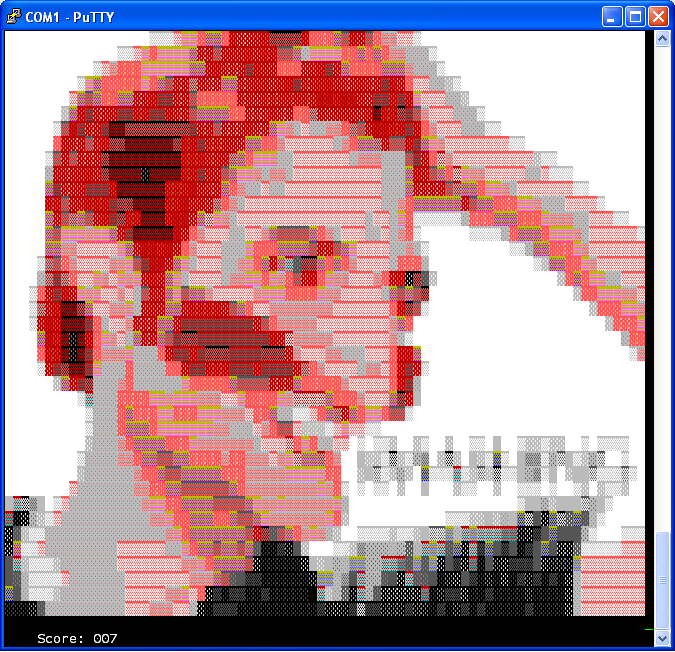
\includegraphics[scale=0.3]{pictures/level_2_complete.PNG}
		\end{subfigure}
		\begin{subfigure}{0.3\linewidth}
			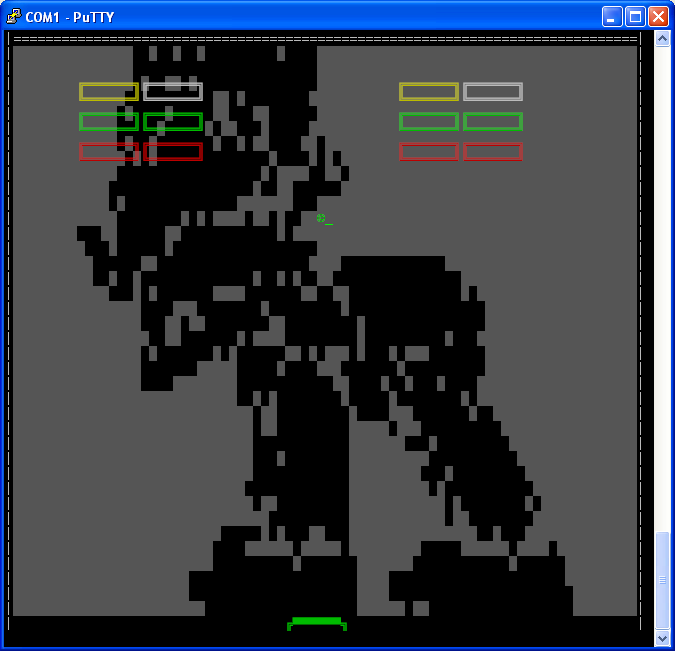
\includegraphics[scale=0.3]{pictures/level_3.PNG}
		\end{subfigure}
		\begin{subfigure}{0.3\linewidth}
			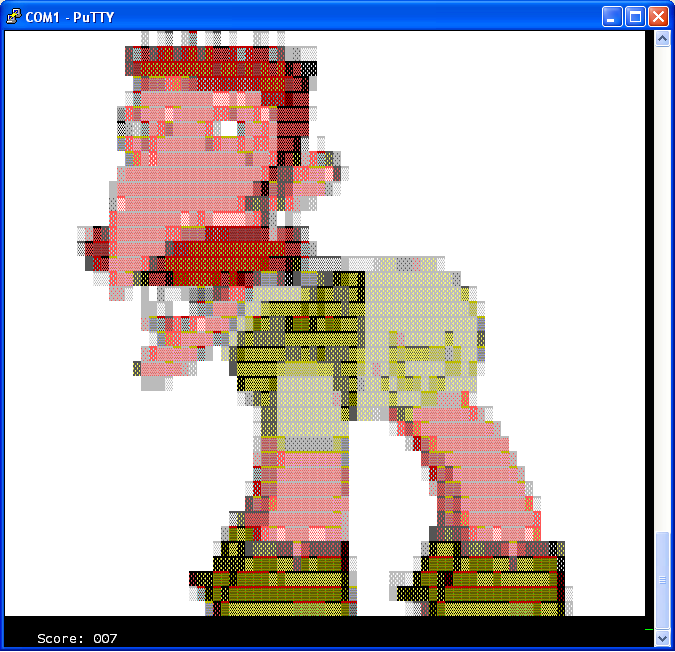
\includegraphics[scale=0.3]{pictures/level_3_complete.PNG}
		\end{subfigure}
	\end{subfigure}
	\begin{subfigure}[b]{\columnwidth}
		\center
		\begin{subfigure}{0.3\linewidth}
			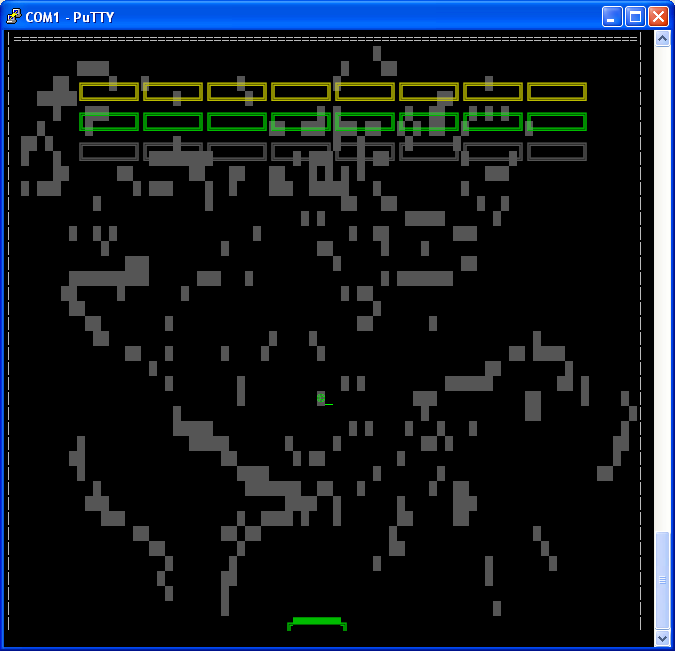
\includegraphics[scale=0.3]{pictures/level_4.PNG}
		\end{subfigure}
		\begin{subfigure}{0.3\linewidth}
			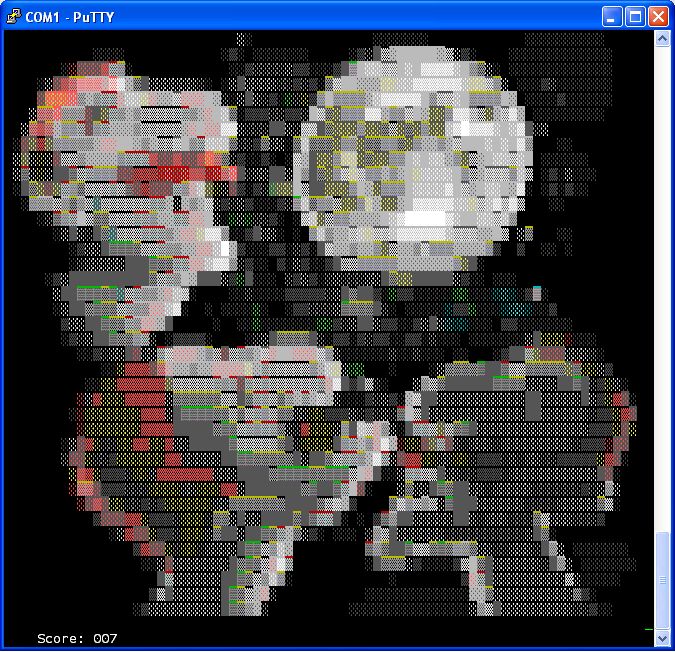
\includegraphics[scale=0.3]{pictures/level_4_complete.PNG}
		\end{subfigure}
		\begin{subfigure}{0.3\linewidth}
			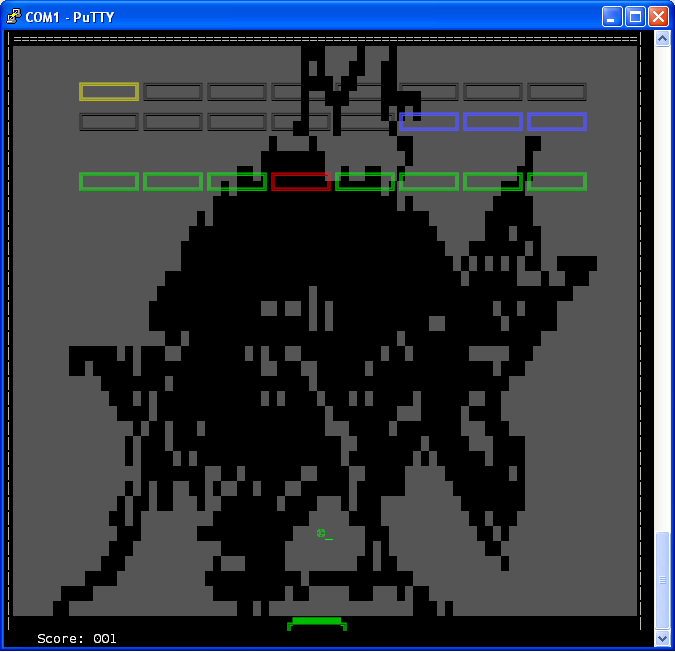
\includegraphics[scale=0.3]{pictures/level_5.PNG}
		\end{subfigure}
	\end{subfigure}
	\caption{Collection of screenshots from Smashing bricks}
	\label{screenshots}
\end{figure}
